\documentclass[tikz,margin=2mm]{standalone}
\pagestyle{empty}

\usepackage{amsmath}
\usepackage{bm}
\usetikzlibrary{positioning,calc, arrows,shapes}

% variable styles
\tikzstyle{measure} = [ draw, rectangle ]
\tikzstyle{latent} = [ draw, ellipse ]


\tikzstyle{edge} = [->]

\begin{document}

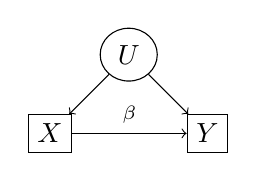
\begin{tikzpicture}
	\node[measure] (x) at (0, 0) {$X$};
	\node[measure] (y) at (2, 0) {$Y$};
	\node[latent] (u) at (1, 1) {$U$};

	\draw[edge](x) -- (y) node[midway, above]{\scriptsize $\beta$};
	\draw[edge](u) -- (x);
	\draw[edge](u) -- (y);
\end{tikzpicture}

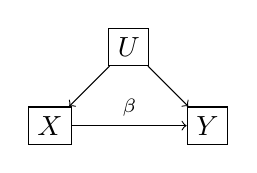
\begin{tikzpicture}
	\node[measure] (x) at (0, 0) {$X$};
	\node[measure] (y) at (2, 0) {$Y$};
	\node[measure] (u) at (1, 1) {$U$};

	\draw[edge](x) -- (y) node[midway, above]{\scriptsize $\beta$};
	\draw[edge](u) -- (x);
	\draw[edge](u) -- (y);
\end{tikzpicture}

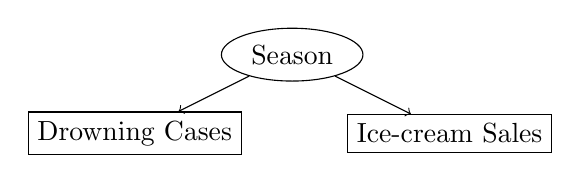
\begin{tikzpicture}
	\node[measure] (x) at (0, 0) {Drowning Cases};
	\node[measure] (y) at (4, 0) {Ice-cream Sales};
	\node[latent] (u) at (2, 1) {Season};

	\draw[edge](u) -- (x);
	\draw[edge](u) -- (y);
\end{tikzpicture}

\end{document}
